\scanpage{67}
$e\longrightarrow I^n$
\[
(\varepsilon_1-\varepsilon_n)
\]
\[
(\varepsilon_1,-\varepsilon_n,x_{n+1}-x_{n+p})
\]
\diagram{\begin{tikzcd}[ampersand replacement=\&]
I^{n+p}\arrow[d,"{x_1-x_n}"]\\ I
\end{tikzcd}}
\figure{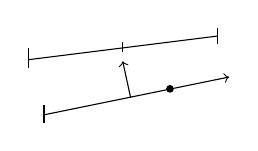
\begin{tikzpicture}
\draw (0,1)--(2.4,1.3); \draw (0,.9)--(0,1.15);
\draw (2.4,1.2)--(2.4,1.4); \draw (1.2,1.1)--(1.2,1.23);
\draw[->] (.2,.3)--(2.55,.78); \draw (.2,.2)--(.2,.43);
\fill (1.8,.63) circle (1.4pt); \draw[->] (1.3,.52)--(1.2,.98);
\end{tikzpicture}}
$(x,y)$\\
$(x',y')$\\
$(x,xy)=(x',x'y')$\\
$\boxed{x=x'}$\\
$xy=x'y'\qquad x=0$\\
$\deleted{x(y-y')=0}$

\diagram{\begin{tikzcd}[ampersand replacement=\&]
I^p\arrow[r]\arrow[d]\&I^{n+p}\arrow[d]\\
\left(\prod_{i\leq n}(\varepsilon_i\times I)\right)^p\times\unsure{e}
\arrow[r,hook]\&(I\times I)^{n\times p}\times I^n
\end{tikzcd}}

$\unsure{x_{ij}}\longleftarrow{}$\\
$f_1,-,f_n\qquad g_1-g_p$\\
$f_i g_j\qquad f'\qquad x_i,x_j$

\diagram{\begin{array}{c}
\boxed{\begin{tikzcd}[ampersand replacement=\&,column sep=large]
\varepsilon_i\times I\arrow[r,hook]\&I\times I
\end{tikzcd}}\\[-4pt]
\begin{tikzcd}[ampersand replacement=\&,column sep=large]
{}\arrow[d]\&{}\arrow[d,"{(x,y)\mapsto(x,xy)}"]\\
e\arrow[r]\&I\times I
\end{tikzcd}
\end{array}}

\diagram{\begin{tikzcd}[ampersand replacement=\&]
I^{n+p}\arrow[d,"{(f_i,g_j)}"']\arrow[dr]\&\\
(\unsure{I^n|I}\times I)^{np}\times\&I^n
\end{tikzcd}}
$f:$ \figure{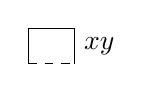
\begin{tikzpicture}[scale=.45]\draw (0,0)--(0,1)--(1.3,1)--(1.3,0);\draw[dashed](0,0)--(1.3,0);\node[right]at(1.3,.5){$xy$};\end{tikzpicture}}

\diagram{\begin{tikzcd}[ampersand replacement=\&]
I^p\arrow[r]\arrow[d]\&I^{n+p}\arrow[d]\\
(\unsure{e}\times I)^{np}\times\unsure{e}\arrow[r,hook]\&(I\times I)^{np}\times I^n
\end{tikzcd}}
\[
(\unsure{e}\times I)^{np}\subset(I\times I)^{np}
\]
a) $0y=0$

\deleted{Dear Fujii Guruji,\\
Please accept my most cordial\\
wishes of welcome in France\\
and of a very happy stay in\\
Paris,}

\diagram{\begin{tikzcd}[ampersand replacement=\&]
X\arrow[r,hook]\arrow[d]\arrow[dr]\&Y\arrow[d]\\
Z\arrow[r,hook]\&I^m
\end{tikzcd}}
comm

\diagram{\begin{tikzcd}[ampersand replacement=\&]
X\arrow[r,hook]\arrow[d]\&Y\arrow[d,"{\varphi=(\varphi_1-\varphi_n)}"]\\
e\arrow[r]\&I^n
\end{tikzcd}}
\deleted{\diagram{\begin{tikzcd}[ampersand replacement=\&]
X\arrow[r,hook]\arrow[d]\&Y\arrow[d,"{\varphi_1-\varphi_{p+n}}"]\\
I^p\arrow[r,hook]\&I^{p+n}
\end{tikzcd}}}
\[
Y\lhook\joinrel\longrightarrow I^p
\qquad \psi=(\psi_1-\psi_p)
\]
\[
\underbrace{(\varphi_i,\psi_j)}_{\chi_{ij}}:Y\longrightarrow(I\times I)^{n\times p}
\]
\deleted{$(\varphi_i,\psi_j)$ se}
$\chi_{ij}|X$ se factorise par $e_i\times I\subset I\times I$

\diagram{\begin{tikzcd}[ampersand replacement=\&]
X\arrow[r,hook]\arrow[d]\&Y\arrow[d]\\
X'=I^p\arrow[r,hook]\arrow[d]\&Y'=I^{n+p}\arrow[d]\\
e\arrow[r,hook]\&S
\arrow[phantom,from=1-1,to=2-2,"{\times}" description]
\arrow[phantom,from=2-1,to=3-2,"{\times}" description]
\end{tikzcd}}
\diagram{\begin{tikzcd}[ampersand replacement=\&]
Y\times Y\arrow[d]\&Y\times_S Y\arrow[l]\arrow[d]\\
Y'\times Y'\arrow[r]\&Y'\times_S Y'
\end{tikzcd}}
$\deleted{\longrightarrow Y\times_{Y'}Y\longrightarrow Y}$
\[
=\overbrace{(\unsure{Y}\times_{Y'}Y)}^{\Delta_{Y/Y'}}\vee(X\times X)
\]
\[
\unsure{\ne}\qquad
\text{``}\Delta_{Y'}\vee(X'\times X')
\]
$I^{\unsure{p}}\ --\ I^{n+p}$\\
$\deleted{\unsure{e\times e\times I^p}}$

\margin{68}
